\documentclass[a4paper, 12pt, french]{article}
\usepackage[utf8]{inputenc}
\usepackage[french]{babel}
\usepackage[T1]{fontenc}
\usepackage[babel=true]{csquotes}
\usepackage{hyperref}
\usepackage{eurosym}
\usepackage{graphicx}
\usepackage{array}
\usepackage{fancyhdr}
\usepackage{lastpage}
\usepackage{xspace}
\usepackage{longtable}
\usepackage{float}
\usepackage{geometry}
\addtolength{\oddsidemargin}{-.875in}
\addtolength{\evensidemargin}{-.875in}
\addtolength{\textwidth}{1.75in}

\addtolength{\topmargin}{-.5in}
\addtolength{\textheight}{1.75in}
%% -- Commandes personalisées

% Contrainte : chaîne de caractères sans espace, en minuscule, constituée seulement des 26 caractères non accentués de l’alphabet latin
\newcommand{\nomProjet}{enflatme\xspace}
% Contrainte : chaîne de caractères sans espace, en minuscule, constituée seulement des 26 caractères non accentués de l’alphabet latin
\newcommand{\nomEquipe}{teamflat\xspace}

\pagestyle{fancy}
% En-têtes
\renewcommand{\headrulewidth}{1pt}
\fancyhead[C]{\nomProjet} 
\fancyhead[L]{Guide utilisateur}
\fancyhead[R]{}

\renewcommand{\footrulewidth}{1pt}
\fancyfoot[C]{Version 1.0} 
\fancyfoot[L]{\nomEquipe\xspace G1}
\fancyfoot[R]{Page \thepage\xspace sur \pageref{LastPage}}

\newcommand{\retourLigne}[2][c]{\begin{tabular}[#1]{@{}l@{}}#2\end{tabular}}

%% -- Document
\begin{document}
	\begin{center}
	    \rule{\linewidth}{1pt}
		\LARGE{\bsc{Guide utilisateur}}
	    \rule{\linewidth}{1pt} \newline{} \newline{}
	\end{center}
	\begin{center}
	    \large{Auteurs :}\\ Antoine \bsc{Augusti} (ANT)\\ Étienne \bsc{Batise} (BAT) \\ Thibaud \bsc{Dauce} (TIB)
	\end{center}
	\vspace{20px}
	\begin{center}
		\large{Date de publication :}\\ \today
	\end{center}

	\section{Connexion à l'application}
	\begin{figure}[H]
    \begin{center}
        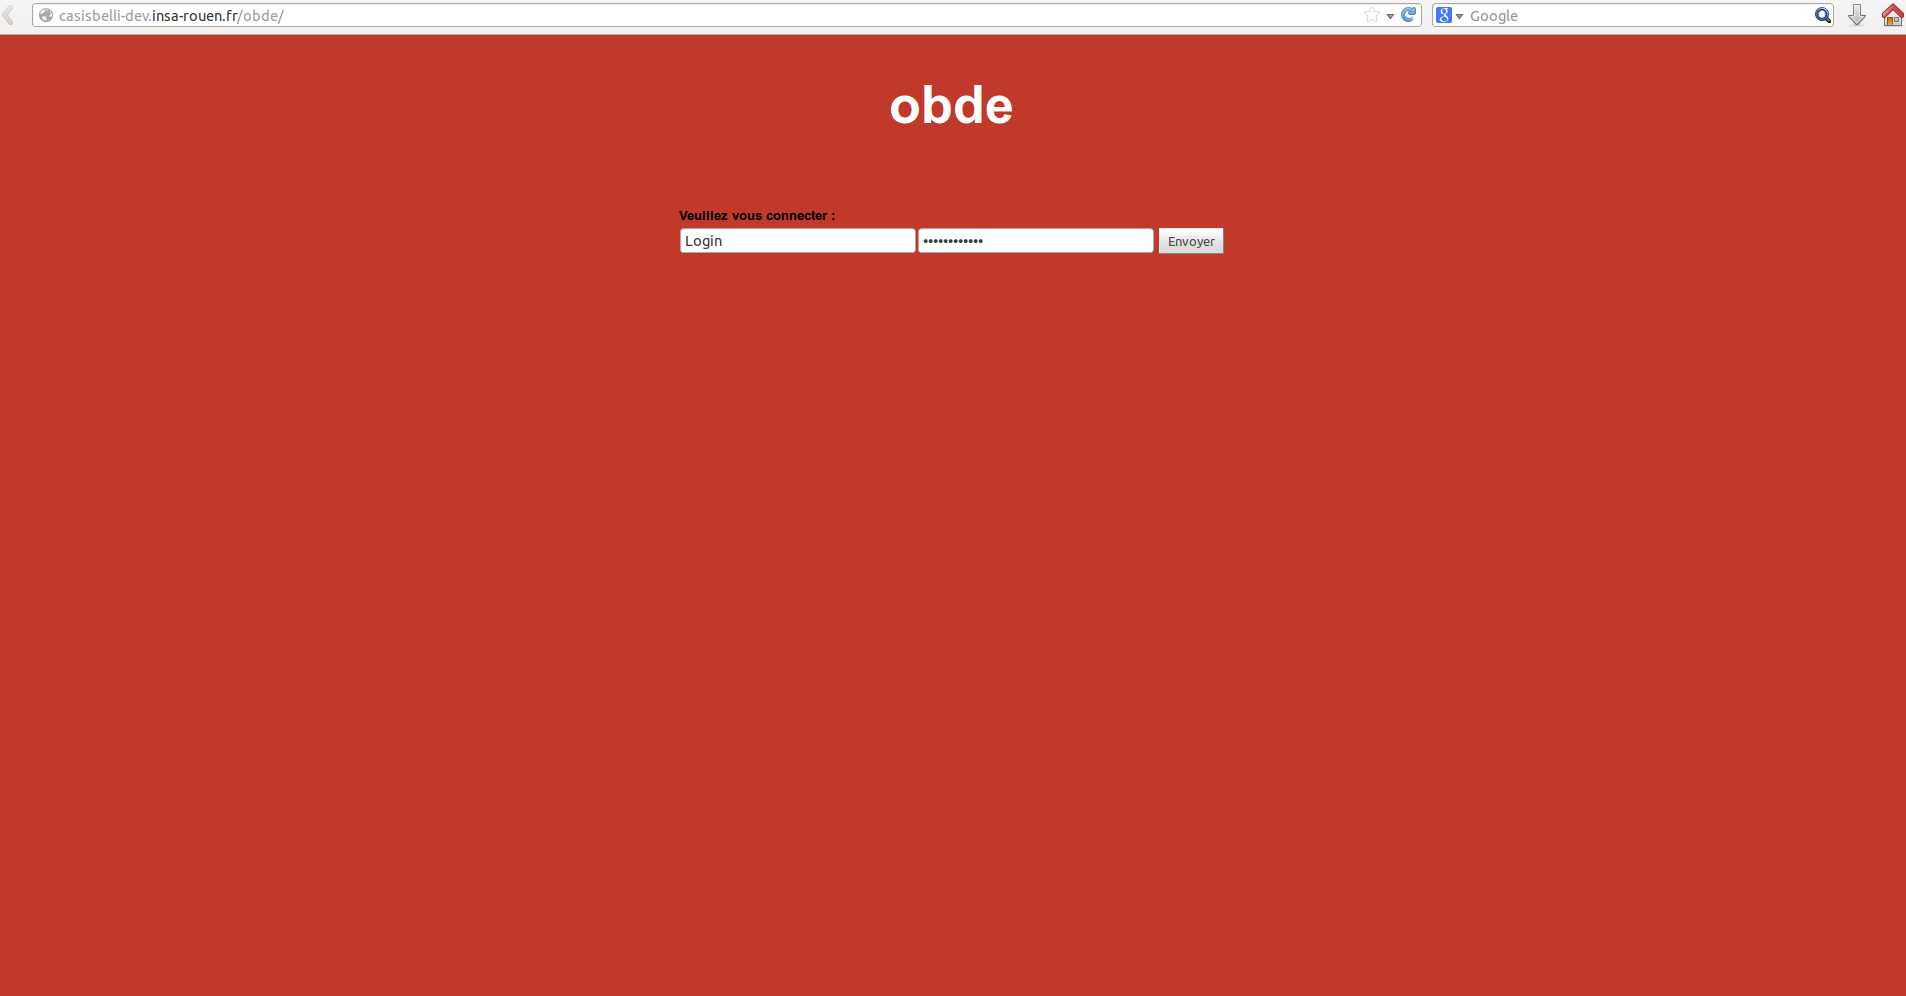
\includegraphics[width=16cm]{screenshoot.png}
    \end{center}
    \caption{Formulaire de connexion de l'application \enquote{obde}}
    \label{img_2}
\end{figure}
	\begin{enumerate}
		\item Rentrer son nom d'utilisateur dans le premier champ texte 
		\item Rentrer son mot de passe dans le deuxième champ texte 
		\item Cliquer sur le bouton \enquote{Envoyer}
	\end{enumerate}

\end{document}